% Generated by analysis/build_report_content.py; edit reviewed JSON and regenerate.
\chapter{Analysis}
\section{General Use cases Diagram}
EPS is an academic escrow simulation for goods and services. Each agreement has one Buyer, one distinct Seller and one full VND amount, funded through a Bank or Payment Gateway mock. The overview is divided into focused views for readability.

\epsfirstfigure{diagrams/overview/UC_General.pdf}{EPS general use case diagram}{fig:overview-uc-general}
\epsfigure{diagrams/overview/UC_Account.pdf}{Account access}{fig:overview-uc-account}
\epsfigure{diagrams/overview/UC_SharedParty.pdf}{Shared escrow-party actions}{fig:overview-uc-sharedparty}
\epsfigure{diagrams/overview/UC_Buyer.pdf}{Buyer journey}{fig:overview-uc-buyer}
\epsfigure{diagrams/overview/UC_Seller.pdf}{Seller journey}{fig:overview-uc-seller}
\epsfigure{diagrams/overview/UC_Admin.pdf}{Administration}{fig:overview-uc-admin}
\epsfigure{diagrams/overview/UC_Payment.pdf}{Payment integration}{fig:overview-uc-payment}
\begin{itemize}
\item \textbf{Guest}: registers an ordinary account and logs in with MFA.
\item \textbf{Buyer}: creates and funds an escrow, accepts delivery and requests release.
\item \textbf{Seller}: accepts the agreement and records delivery or service completion. Both participants may request a refund or open a dispute.
\item \textbf{Admin}: resolves disputes, updates policy, views analytics/audit and reconciles pending transfers.
\item \textbf{Merchant/Marketplace}: creates and queries only its own escrows through a separately authenticated client.
\item \textbf{Partner Bank}: simulates funding, Seller release and refunds for Bank-funded escrows.
\item \textbf{Payment Gateway}: simulates funding and refunds to the original Gateway source.
\end{itemize}
Buyer and Seller are roles in each transaction. Release uses the Bank mock; refund returns through the original funding provider. Real money, partial payments, milestones and automatic release are outside this MVP.

\section{Use case Details}
\par\begingroup\ifdim\dimexpr\pagegoal-\pagetotal\relax<180pt\relax\newpage\fi\endgroup
\subsection{User's Use cases Details}
\par\begingroup\ifdim\dimexpr\pagegoal-\pagetotal\relax<120pt\relax\newpage\fi\endgroup\medskip\noindent\textbf{U1: Register}
{\fontsize{10.5}{13}\selectfont\setlength{\tabcolsep}{4pt}
\begin{longtable}{|>{\raggedright\arraybackslash}p{0.22\linewidth}|>{\raggedright\arraybackslash}p{0.07\linewidth}|>{\raggedright\arraybackslash}p{0.17\linewidth}|>{\raggedright\arraybackslash}p{0.44\linewidth}|}
\hline\endfirsthead
\multicolumn{4}{|l|}{\textit{U1 (continued)}}\\\hline\endhead
\endfoot\endlastfoot
\textbf{Use Case Code} & U1 & \textbf{Use Case Name} & Register \\\hline
\textbf{Actor} & \multicolumn{3}{p{\dimexpr0.68\linewidth+4\tabcolsep+2\arrayrulewidth\relax}|}{Guest} \\\hline
\textbf{Usage} & \multicolumn{3}{p{\dimexpr0.68\linewidth+4\tabcolsep+2\arrayrulewidth\relax}|}{Create an ordinary user account.} \\\hline
\textbf{Activation Event} & \multicolumn{3}{p{\dimexpr0.68\linewidth+4\tabcolsep+2\arrayrulewidth\relax}|}{Guest selects Register.} \\\hline
\textbf{Preconditions} & \multicolumn{3}{p{\dimexpr0.68\linewidth+4\tabcolsep+2\arrayrulewidth\relax}|}{The login identifier is not already registered.} \\\hline
\textbf{Main Event Flow} & \textbf{Index} & \textbf{Done by} & \textbf{Action} \\\hline
 & 1 & Guest & Enter account details and password. \\\hline
 & 2 & EPS & Validate the details and start MFA enrollment; do not grant Admin or Merchant privileges. \\\hline
 & 3 & Guest & Complete the MFA enrollment challenge. \\\hline
 & 4 & EPS & Create the account after successful verification and direct the user to Login. \\\hline
 & 5 & EPS & For invalid details, a duplicate identifier or failed MFA, reject registration without activating an account. \\\hline
\textbf{Postconditions} & \multicolumn{3}{p{\dimexpr0.68\linewidth+4\tabcolsep+2\arrayrulewidth\relax}|}{A valid ordinary account is created; the user must log in separately.} \\\hline
\end{longtable}}
\par\begingroup\ifdim\dimexpr\pagegoal-\pagetotal\relax<120pt\relax\newpage\fi\endgroup\medskip\noindent\textbf{U2: Login with MFA}
{\fontsize{10.5}{13}\selectfont\setlength{\tabcolsep}{4pt}
\begin{longtable}{|>{\raggedright\arraybackslash}p{0.22\linewidth}|>{\raggedright\arraybackslash}p{0.07\linewidth}|>{\raggedright\arraybackslash}p{0.17\linewidth}|>{\raggedright\arraybackslash}p{0.44\linewidth}|}
\hline\endfirsthead
\multicolumn{4}{|l|}{\textit{U2 (continued)}}\\\hline\endhead
\endfoot\endlastfoot
\textbf{Use Case Code} & U2 & \textbf{Use Case Name} & Login with MFA \\\hline
\textbf{Actor} & \multicolumn{3}{p{\dimexpr0.68\linewidth+4\tabcolsep+2\arrayrulewidth\relax}|}{Buyer; Seller; Admin} \\\hline
\textbf{Usage} & \multicolumn{3}{p{\dimexpr0.68\linewidth+4\tabcolsep+2\arrayrulewidth\relax}|}{Start an authenticated user session.} \\\hline
\textbf{Activation Event} & \multicolumn{3}{p{\dimexpr0.68\linewidth+4\tabcolsep+2\arrayrulewidth\relax}|}{User selects Login.} \\\hline
\textbf{Preconditions} & \multicolumn{3}{p{\dimexpr0.68\linewidth+4\tabcolsep+2\arrayrulewidth\relax}|}{An active user or pre-provisioned Admin account exists.} \\\hline
\textbf{Main Event Flow} & \textbf{Index} & \textbf{Done by} & \textbf{Action} \\\hline
 & 1 & User & Submit the login identifier and password. \\\hline
 & 2 & EPS & Verify credentials and request the enrolled MFA factor. \\\hline
 & 3 & User & Submit the MFA response. \\\hline
 & 4 & EPS & Verify MFA, create the session and show the permitted workspace. \\\hline
 & 5 & EPS & Reject invalid credentials or MFA without creating a session. Merchant client credentials cannot be used as a human login. \\\hline
\textbf{Postconditions} & \multicolumn{3}{p{\dimexpr0.68\linewidth+4\tabcolsep+2\arrayrulewidth\relax}|}{A successful login creates a session with the account's existing permissions.} \\\hline
\end{longtable}}
\par\begingroup\ifdim\dimexpr\pagegoal-\pagetotal\relax<120pt\relax\newpage\fi\endgroup\medskip\noindent\textbf{U3: Logout}
{\fontsize{10.5}{13}\selectfont\setlength{\tabcolsep}{4pt}
\begin{longtable}{|>{\raggedright\arraybackslash}p{0.22\linewidth}|>{\raggedright\arraybackslash}p{0.07\linewidth}|>{\raggedright\arraybackslash}p{0.17\linewidth}|>{\raggedright\arraybackslash}p{0.44\linewidth}|}
\hline\endfirsthead
\multicolumn{4}{|l|}{\textit{U3 (continued)}}\\\hline\endhead
\endfoot\endlastfoot
\textbf{Use Case Code} & U3 & \textbf{Use Case Name} & Logout \\\hline
\textbf{Actor} & \multicolumn{3}{p{\dimexpr0.68\linewidth+4\tabcolsep+2\arrayrulewidth\relax}|}{Buyer; Seller; Admin} \\\hline
\textbf{Usage} & \multicolumn{3}{p{\dimexpr0.68\linewidth+4\tabcolsep+2\arrayrulewidth\relax}|}{End the current user session.} \\\hline
\textbf{Activation Event} & \multicolumn{3}{p{\dimexpr0.68\linewidth+4\tabcolsep+2\arrayrulewidth\relax}|}{User selects Logout.} \\\hline
\textbf{Preconditions} & \multicolumn{3}{p{\dimexpr0.68\linewidth+4\tabcolsep+2\arrayrulewidth\relax}|}{A current or previously expired session is available.} \\\hline
\textbf{Main Event Flow} & \textbf{Index} & \textbf{Done by} & \textbf{Action} \\\hline
 & 1 & User & Select Logout. \\\hline
 & 2 & EPS & Invalidate the current session and show Login. An already expired session returns the same result. \\\hline
\textbf{Postconditions} & \multicolumn{3}{p{\dimexpr0.68\linewidth+4\tabcolsep+2\arrayrulewidth\relax}|}{The previous session cannot access protected functions.} \\\hline
\end{longtable}}
\par\begingroup\ifdim\dimexpr\pagegoal-\pagetotal\relax<120pt\relax\newpage\fi\endgroup\medskip\noindent\textbf{U4: View/Track Escrows}
{\fontsize{10.5}{13}\selectfont\setlength{\tabcolsep}{4pt}
\begin{longtable}{|>{\raggedright\arraybackslash}p{0.22\linewidth}|>{\raggedright\arraybackslash}p{0.07\linewidth}|>{\raggedright\arraybackslash}p{0.17\linewidth}|>{\raggedright\arraybackslash}p{0.44\linewidth}|}
\hline\endfirsthead
\multicolumn{4}{|l|}{\textit{U4 (continued)}}\\\hline\endhead
\endfoot\endlastfoot
\textbf{Use Case Code} & U4 & \textbf{Use Case Name} & View/Track Escrows \\\hline
\textbf{Actor} & \multicolumn{3}{p{\dimexpr0.68\linewidth+4\tabcolsep+2\arrayrulewidth\relax}|}{Buyer; Seller; Merchant/Marketplace (U4.API variant)} \\\hline
\textbf{Usage} & \multicolumn{3}{p{\dimexpr0.68\linewidth+4\tabcolsep+2\arrayrulewidth\relax}|}{View escrows and their current progress.} \\\hline
\textbf{Activation Event} & \multicolumn{3}{p{\dimexpr0.68\linewidth+4\tabcolsep+2\arrayrulewidth\relax}|}{User opens the escrow list or an escrow detail.} \\\hline
\textbf{Preconditions} & \multicolumn{3}{p{\dimexpr0.68\linewidth+4\tabcolsep+2\arrayrulewidth\relax}|}{The user is authenticated and is a participant in the requested escrow.} \\\hline
\textbf{Main Event Flow} & \textbf{Index} & \textbf{Done by} & \textbf{Action} \\\hline
 & 1 & User & Request the list or select an escrow. \\\hline
 & 2 & EPS & Check access and retrieve the authorised record. \\\hline
 & 3 & EPS & Show terms, lifecycle, payment status, delivery, refund proposal and dispute status. \\\hline
 & 4 & EPS & Show unresolved operations as pending with a query reference; viewing does not move money. \\\hline
 & 5 & EPS & Reject access to another user's escrow without disclosing its data. \\\hline
 & API & Merchant & U4.API: Authenticate the Merchant client and return only its owned escrow status. Pending results include a query reference. Reject other clients' escrows and exclude private dispute evidence and Admin audit data. \\\hline
\textbf{Postconditions} & \multicolumn{3}{p{\dimexpr0.68\linewidth+4\tabcolsep+2\arrayrulewidth\relax}|}{The authorised current status is displayed; the escrow is unchanged.} \\\hline
\end{longtable}}
\par\begingroup\ifdim\dimexpr\pagegoal-\pagetotal\relax<120pt\relax\newpage\fi\endgroup\medskip\noindent\textbf{U5: Open Dispute}
{\fontsize{10.5}{13}\selectfont\setlength{\tabcolsep}{4pt}
\begin{longtable}{|>{\raggedright\arraybackslash}p{0.22\linewidth}|>{\raggedright\arraybackslash}p{0.07\linewidth}|>{\raggedright\arraybackslash}p{0.17\linewidth}|>{\raggedright\arraybackslash}p{0.44\linewidth}|}
\hline\endfirsthead
\multicolumn{4}{|l|}{\textit{U5 (continued)}}\\\hline\endhead
\endfoot\endlastfoot
\textbf{Use Case Code} & U5 & \textbf{Use Case Name} & Open Dispute \\\hline
\textbf{Actor} & \multicolumn{3}{p{\dimexpr0.68\linewidth+4\tabcolsep+2\arrayrulewidth\relax}|}{Buyer; Seller} \\\hline
\textbf{Usage} & \multicolumn{3}{p{\dimexpr0.68\linewidth+4\tabcolsep+2\arrayrulewidth\relax}|}{Request Admin resolution of a held escrow.} \\\hline
\textbf{Activation Event} & \multicolumn{3}{p{\dimexpr0.68\linewidth+4\tabcolsep+2\arrayrulewidth\relax}|}{Buyer or Seller selects Open Dispute.} \\\hline
\textbf{Preconditions} & \multicolumn{3}{p{\dimexpr0.68\linewidth+4\tabcolsep+2\arrayrulewidth\relax}|}{The escrow is HELD or DELIVERED; no dispute has previously been opened and no payout is reserved.} \\\hline
\textbf{Main Event Flow} & \textbf{Index} & \textbf{Done by} & \textbf{Action} \\\hline
 & 1 & Buyer/Seller & Enter the dispute reason. \\\hline
 & 2 & EPS & Recheck participant access and dispute eligibility. \\\hline
 & 3 & EPS & Open the dispute and invalidate any pending refund proposal in one state change. \\\hline
 & 4 & EPS & Save the case and allow both parties to submit evidence; block delivery and ordinary release. \\\hline
 & 5 & EPS & Reject a stale or concurrent request if another payout or dispute decision has already been accepted. \\\hline
\textbf{Postconditions} & \multicolumn{3}{p{\dimexpr0.68\linewidth+4\tabcolsep+2\arrayrulewidth\relax}|}{One OPEN dispute exists; the full amount remains held.} \\\hline
\end{longtable}}
\par\begingroup\ifdim\dimexpr\pagegoal-\pagetotal\relax<120pt\relax\newpage\fi\endgroup\medskip\noindent\textbf{U6: Submit Dispute Evidence}
{\fontsize{10.5}{13}\selectfont\setlength{\tabcolsep}{4pt}
\begin{longtable}{|>{\raggedright\arraybackslash}p{0.22\linewidth}|>{\raggedright\arraybackslash}p{0.07\linewidth}|>{\raggedright\arraybackslash}p{0.17\linewidth}|>{\raggedright\arraybackslash}p{0.44\linewidth}|}
\hline\endfirsthead
\multicolumn{4}{|l|}{\textit{U6 (continued)}}\\\hline\endhead
\endfoot\endlastfoot
\textbf{Use Case Code} & U6 & \textbf{Use Case Name} & Submit Dispute Evidence \\\hline
\textbf{Actor} & \multicolumn{3}{p{\dimexpr0.68\linewidth+4\tabcolsep+2\arrayrulewidth\relax}|}{Buyer; Seller} \\\hline
\textbf{Usage} & \multicolumn{3}{p{\dimexpr0.68\linewidth+4\tabcolsep+2\arrayrulewidth\relax}|}{Add evidence to an open dispute.} \\\hline
\textbf{Activation Event} & \multicolumn{3}{p{\dimexpr0.68\linewidth+4\tabcolsep+2\arrayrulewidth\relax}|}{A participant selects Submit Evidence.} \\\hline
\textbf{Preconditions} & \multicolumn{3}{p{\dimexpr0.68\linewidth+4\tabcolsep+2\arrayrulewidth\relax}|}{The participant belongs to the escrow and the dispute remains OPEN.} \\\hline
\textbf{Main Event Flow} & \textbf{Index} & \textbf{Done by} & \textbf{Action} \\\hline
 & 1 & Buyer/Seller & Submit evidence and a short explanation. \\\hline
 & 2 & EPS & Validate the submission and recheck that no final decision has been recorded. \\\hline
 & 3 & EPS & Save the evidence with its author and submission time. \\\hline
 & 4 & EPS & Reject unauthorised submissions or evidence received after the final decision. \\\hline
\textbf{Postconditions} & \multicolumn{3}{p{\dimexpr0.68\linewidth+4\tabcolsep+2\arrayrulewidth\relax}|}{Accepted evidence is available for dispute review.} \\\hline
\end{longtable}}
\par\begingroup\ifdim\dimexpr\pagegoal-\pagetotal\relax<120pt\relax\newpage\fi\endgroup\medskip\noindent\textbf{U7: Propose/Withdraw Full Refund}
{\fontsize{10.5}{13}\selectfont\setlength{\tabcolsep}{4pt}
\begin{longtable}{|>{\raggedright\arraybackslash}p{0.22\linewidth}|>{\raggedright\arraybackslash}p{0.07\linewidth}|>{\raggedright\arraybackslash}p{0.17\linewidth}|>{\raggedright\arraybackslash}p{0.44\linewidth}|}
\hline\endfirsthead
\multicolumn{4}{|l|}{\textit{U7 (continued)}}\\\hline\endhead
\endfoot\endlastfoot
\textbf{Use Case Code} & U7 & \textbf{Use Case Name} & Propose/Withdraw Full Refund \\\hline
\textbf{Actor} & \multicolumn{3}{p{\dimexpr0.68\linewidth+4\tabcolsep+2\arrayrulewidth\relax}|}{Buyer; Seller} \\\hline
\textbf{Usage} & \multicolumn{3}{p{\dimexpr0.68\linewidth+4\tabcolsep+2\arrayrulewidth\relax}|}{Propose or withdraw a full refund.} \\\hline
\textbf{Activation Event} & \multicolumn{3}{p{\dimexpr0.68\linewidth+4\tabcolsep+2\arrayrulewidth\relax}|}{A participant selects Propose Refund or Withdraw Proposal.} \\\hline
\textbf{Preconditions} & \multicolumn{3}{p{\dimexpr0.68\linewidth+4\tabcolsep+2\arrayrulewidth\relax}|}{The escrow is HELD or DELIVERED, with no open dispute or reserved payout.} \\\hline
\textbf{Main Event Flow} & \textbf{Index} & \textbf{Done by} & \textbf{Action} \\\hline
 & 1 & Buyer/Seller & Submit a full-refund reason, or select their pending proposal for withdrawal. \\\hline
 & 2 & EPS & For a new proposal, check that no other proposal is pending; save it and notify the counterpart. \\\hline
 & 3 & EPS & While the proposal is pending, block new delivery recording and ordinary Buyer release. \\\hline
 & 4 & EPS & Allow only the proposer to withdraw before approval. Restore otherwise eligible actions without deleting saved delivery. \\\hline
 & 5 & EPS & Reject stale requests; repeated requests return the recorded result. \\\hline
\textbf{Postconditions} & \multicolumn{3}{p{\dimexpr0.68\linewidth+4\tabcolsep+2\arrayrulewidth\relax}|}{The proposal is PENDING or WITHDRAWN; no money is transferred.} \\\hline
\end{longtable}}
\par\begingroup\ifdim\dimexpr\pagegoal-\pagetotal\relax<120pt\relax\newpage\fi\endgroup\medskip\noindent\textbf{U8: Accept/Reject Refund Proposal}
{\fontsize{10.5}{13}\selectfont\setlength{\tabcolsep}{4pt}
\begin{longtable}{|>{\raggedright\arraybackslash}p{0.22\linewidth}|>{\raggedright\arraybackslash}p{0.07\linewidth}|>{\raggedright\arraybackslash}p{0.17\linewidth}|>{\raggedright\arraybackslash}p{0.44\linewidth}|}
\hline\endfirsthead
\multicolumn{4}{|l|}{\textit{U8 (continued)}}\\\hline\endhead
\endfoot\endlastfoot
\textbf{Use Case Code} & U8 & \textbf{Use Case Name} & Accept/Reject Refund Proposal \\\hline
\textbf{Actor} & \multicolumn{3}{p{\dimexpr0.68\linewidth+4\tabcolsep+2\arrayrulewidth\relax}|}{Buyer; Seller} \\\hline
\textbf{Usage} & \multicolumn{3}{p{\dimexpr0.68\linewidth+4\tabcolsep+2\arrayrulewidth\relax}|}{Accept or reject the counterpart's full-refund proposal.} \\\hline
\textbf{Activation Event} & \multicolumn{3}{p{\dimexpr0.68\linewidth+4\tabcolsep+2\arrayrulewidth\relax}|}{The counterpart responds to a proposal.} \\\hline
\textbf{Preconditions} & \multicolumn{3}{p{\dimexpr0.68\linewidth+4\tabcolsep+2\arrayrulewidth\relax}|}{The proposal is PENDING and the escrow has no open dispute or reserved payout.} \\\hline
\textbf{Main Event Flow} & \textbf{Index} & \textbf{Done by} & \textbf{Action} \\\hline
 & 1 & Buyer/Seller & Review the proposal and choose Accept or Reject. \\\hline
 & 2 & EPS & Recheck that the responder is the counterpart and the proposal remains eligible. \\\hline
 & 3 & EPS & On acceptance, approve the proposal and reserve the full refund as REFUND\_\allowbreak{}PENDING; invoke P3. \\\hline
 & 4 & EPS & On rejection, mark REJECTED and restore otherwise eligible actions without reverting delivery. \\\hline
 & 5 & EPS & Reject self-approval or a stale response. A repeated response returns the recorded result. \\\hline
\textbf{Postconditions} & \multicolumn{3}{p{\dimexpr0.68\linewidth+4\tabcolsep+2\arrayrulewidth\relax}|}{Approval starts P3; rejection makes no payment. Only confirmed provider success produces REFUNDED.} \\\hline
\end{longtable}}
\par\begingroup\ifdim\dimexpr\pagegoal-\pagetotal\relax<180pt\relax\newpage\fi\endgroup
\subsection{Buyer's Use cases Details}
\par\begingroup\ifdim\dimexpr\pagegoal-\pagetotal\relax<120pt\relax\newpage\fi\endgroup\medskip\noindent\textbf{B1: Create Escrow}
{\fontsize{10.5}{13}\selectfont\setlength{\tabcolsep}{4pt}
\begin{longtable}{|>{\raggedright\arraybackslash}p{0.22\linewidth}|>{\raggedright\arraybackslash}p{0.07\linewidth}|>{\raggedright\arraybackslash}p{0.17\linewidth}|>{\raggedright\arraybackslash}p{0.44\linewidth}|}
\hline\endfirsthead
\multicolumn{4}{|l|}{\textit{B1 (continued)}}\\\hline\endhead
\endfoot\endlastfoot
\textbf{Use Case Code} & B1 & \textbf{Use Case Name} & Create Escrow \\\hline
\textbf{Actor} & \multicolumn{3}{p{\dimexpr0.68\linewidth+4\tabcolsep+2\arrayrulewidth\relax}|}{Buyer; Merchant/Marketplace (B1.API variant)} \\\hline
\textbf{Usage} & \multicolumn{3}{p{\dimexpr0.68\linewidth+4\tabcolsep+2\arrayrulewidth\relax}|}{Create an escrow agreement.} \\\hline
\textbf{Activation Event} & \multicolumn{3}{p{\dimexpr0.68\linewidth+4\tabcolsep+2\arrayrulewidth\relax}|}{Buyer selects Create Escrow.} \\\hline
\textbf{Preconditions} & \multicolumn{3}{p{\dimexpr0.68\linewidth+4\tabcolsep+2\arrayrulewidth\relax}|}{The Buyer is authenticated; the Buyer and Seller are distinct existing users.} \\\hline
\textbf{Main Event Flow} & \textbf{Index} & \textbf{Done by} & \textbf{Action} \\\hline
 & 1 & Buyer & Enter the Seller, GOODS/SERVICES, full VND amount, deliverable and acceptance criteria. \\\hline
 & 2 & EPS & Validate the agreement and capture the current evidence policy and Seller destination. \\\hline
 & 3 & EPS & Save the escrow as AWAITING\_\allowbreak{}SELLER and notify the Seller. \\\hline
 & 4 & EPS & Reject invalid terms or self-trading. An identical repeated creation returns the existing escrow. \\\hline
 & API & Merchant & B1.API: Authenticate the Merchant client, use its bound Seller and validate the same B1 terms. Save client ownership and return the escrow reference and AWAITING\_\allowbreak{}SELLER. Reject another Seller or conflicting request reuse; identical repeats return the existing escrow. \\\hline
\textbf{Postconditions} & \multicolumn{3}{p{\dimexpr0.68\linewidth+4\tabcolsep+2\arrayrulewidth\relax}|}{The agreement awaits Seller acceptance; no funding has started.} \\\hline
\end{longtable}}
\par\begingroup\ifdim\dimexpr\pagegoal-\pagetotal\relax<120pt\relax\newpage\fi\endgroup\medskip\noindent\textbf{B2: Cancel Unfunded Escrow}
{\fontsize{10.5}{13}\selectfont\setlength{\tabcolsep}{4pt}
\begin{longtable}{|>{\raggedright\arraybackslash}p{0.22\linewidth}|>{\raggedright\arraybackslash}p{0.07\linewidth}|>{\raggedright\arraybackslash}p{0.17\linewidth}|>{\raggedright\arraybackslash}p{0.44\linewidth}|}
\hline\endfirsthead
\multicolumn{4}{|l|}{\textit{B2 (continued)}}\\\hline\endhead
\endfoot\endlastfoot
\textbf{Use Case Code} & B2 & \textbf{Use Case Name} & Cancel Unfunded Escrow \\\hline
\textbf{Actor} & \multicolumn{3}{p{\dimexpr0.68\linewidth+4\tabcolsep+2\arrayrulewidth\relax}|}{Buyer} \\\hline
\textbf{Usage} & \multicolumn{3}{p{\dimexpr0.68\linewidth+4\tabcolsep+2\arrayrulewidth\relax}|}{Cancel an escrow before funding.} \\\hline
\textbf{Activation Event} & \multicolumn{3}{p{\dimexpr0.68\linewidth+4\tabcolsep+2\arrayrulewidth\relax}|}{Buyer selects Cancel.} \\\hline
\textbf{Preconditions} & \multicolumn{3}{p{\dimexpr0.68\linewidth+4\tabcolsep+2\arrayrulewidth\relax}|}{The escrow is AWAITING\_\allowbreak{}SELLER or AWAITING\_\allowbreak{}FUNDING; no money was received and no funding result is unresolved.} \\\hline
\textbf{Main Event Flow} & \textbf{Index} & \textbf{Done by} & \textbf{Action} \\\hline
 & 1 & Buyer & Confirm cancellation of their escrow. \\\hline
 & 2 & EPS & Recheck ownership and funding status. \\\hline
 & 3 & EPS & Set CANCELLED and record the reason. \\\hline
 & 4 & EPS & Reject cancellation while funding is active or unknown. A repeated cancellation returns the existing result. \\\hline
\textbf{Postconditions} & \multicolumn{3}{p{\dimexpr0.68\linewidth+4\tabcolsep+2\arrayrulewidth\relax}|}{The cancelled escrow cannot accept funding or payout.} \\\hline
\end{longtable}}
\par\begingroup\ifdim\dimexpr\pagegoal-\pagetotal\relax<120pt\relax\newpage\fi\endgroup\medskip\noindent\textbf{B3: Fund Escrow}
{\fontsize{10.5}{13}\selectfont\setlength{\tabcolsep}{4pt}
\begin{longtable}{|>{\raggedright\arraybackslash}p{0.22\linewidth}|>{\raggedright\arraybackslash}p{0.07\linewidth}|>{\raggedright\arraybackslash}p{0.17\linewidth}|>{\raggedright\arraybackslash}p{0.44\linewidth}|}
\hline\endfirsthead
\multicolumn{4}{|l|}{\textit{B3 (continued)}}\\\hline\endhead
\endfoot\endlastfoot
\textbf{Use Case Code} & B3 & \textbf{Use Case Name} & Fund Escrow \\\hline
\textbf{Actor} & \multicolumn{3}{p{\dimexpr0.68\linewidth+4\tabcolsep+2\arrayrulewidth\relax}|}{Buyer; Partner Bank; Payment Gateway} \\\hline
\textbf{Usage} & \multicolumn{3}{p{\dimexpr0.68\linewidth+4\tabcolsep+2\arrayrulewidth\relax}|}{Fund the full accepted agreement through a mock provider.} \\\hline
\textbf{Activation Event} & \multicolumn{3}{p{\dimexpr0.68\linewidth+4\tabcolsep+2\arrayrulewidth\relax}|}{Buyer selects Fund Escrow.} \\\hline
\textbf{Preconditions} & \multicolumn{3}{p{\dimexpr0.68\linewidth+4\tabcolsep+2\arrayrulewidth\relax}|}{Seller has accepted; the escrow is AWAITING\_\allowbreak{}FUNDING with no unresolved funding attempt.} \\\hline
\textbf{Main Event Flow} & \textbf{Index} & \textbf{Done by} & \textbf{Action} \\\hline
 & 1 & Buyer & Review the terms, accept them and choose Bank or Gateway. \\\hline
 & 2 & EPS & Save a funding reference and set FUNDING\_\allowbreak{}PENDING. \\\hline
 & 3 & Bank/Gateway & Process the full VND funding request and return a result through P1. \\\hline
 & 4 & EPS & Show the confirmed result, or keep pending if the result is uncertain. \\\hline
 & 5 & EPS & Only confirmed failure with no receipt returns AWAITING\_\allowbreak{}FUNDING, allowing the Buyer to retry or cancel. \\\hline
\textbf{Postconditions} & \multicolumn{3}{p{\dimexpr0.68\linewidth+4\tabcolsep+2\arrayrulewidth\relax}|}{Only P1 confirmation establishes HELD. A timeout does not permit another funding attempt.} \\\hline
\end{longtable}}
\par\begingroup\ifdim\dimexpr\pagegoal-\pagetotal\relax<120pt\relax\newpage\fi\endgroup\medskip\noindent\textbf{B4: Confirm Acceptance and Request Release}
{\fontsize{10.5}{13}\selectfont\setlength{\tabcolsep}{4pt}
\begin{longtable}{|>{\raggedright\arraybackslash}p{0.22\linewidth}|>{\raggedright\arraybackslash}p{0.07\linewidth}|>{\raggedright\arraybackslash}p{0.17\linewidth}|>{\raggedright\arraybackslash}p{0.44\linewidth}|}
\hline\endfirsthead
\multicolumn{4}{|l|}{\textit{B4 (continued)}}\\\hline\endhead
\endfoot\endlastfoot
\textbf{Use Case Code} & B4 & \textbf{Use Case Name} & Confirm Acceptance and Request Release \\\hline
\textbf{Actor} & \multicolumn{3}{p{\dimexpr0.68\linewidth+4\tabcolsep+2\arrayrulewidth\relax}|}{Buyer; Partner Bank} \\\hline
\textbf{Usage} & \multicolumn{3}{p{\dimexpr0.68\linewidth+4\tabcolsep+2\arrayrulewidth\relax}|}{Accept delivery and request full release to the Seller.} \\\hline
\textbf{Activation Event} & \multicolumn{3}{p{\dimexpr0.68\linewidth+4\tabcolsep+2\arrayrulewidth\relax}|}{Buyer selects Confirm Acceptance.} \\\hline
\textbf{Preconditions} & \multicolumn{3}{p{\dimexpr0.68\linewidth+4\tabcolsep+2\arrayrulewidth\relax}|}{The escrow is DELIVERED and its evidence policy is satisfied; no refund proposal, open dispute or payout is pending.} \\\hline
\textbf{Main Event Flow} & \textbf{Index} & \textbf{Done by} & \textbf{Action} \\\hline
 & 1 & Buyer & Review delivery and confirm acceptance. \\\hline
 & 2 & EPS & Recheck access, evidence and escrow eligibility. \\\hline
 & 3 & EPS & Reserve the full amount as RELEASE\_\allowbreak{}PENDING and invoke P2 through the Bank mock. \\\hline
 & 4 & EPS & Show the pending or confirmed result. \\\hline
 & 5 & EPS & Reject a conflicting request; a repeated acceptance returns the saved release decision. \\\hline
\textbf{Postconditions} & \multicolumn{3}{p{\dimexpr0.68\linewidth+4\tabcolsep+2\arrayrulewidth\relax}|}{Release is requested once. RELEASED requires confirmed Bank settlement.} \\\hline
\end{longtable}}
\par\begingroup\ifdim\dimexpr\pagegoal-\pagetotal\relax<180pt\relax\newpage\fi\endgroup
\subsection{Seller's Use cases Details}
\par\begingroup\ifdim\dimexpr\pagegoal-\pagetotal\relax<120pt\relax\newpage\fi\endgroup\medskip\noindent\textbf{S1: Accept/Reject Escrow Terms}
{\fontsize{10.5}{13}\selectfont\setlength{\tabcolsep}{4pt}
\begin{longtable}{|>{\raggedright\arraybackslash}p{0.22\linewidth}|>{\raggedright\arraybackslash}p{0.07\linewidth}|>{\raggedright\arraybackslash}p{0.17\linewidth}|>{\raggedright\arraybackslash}p{0.44\linewidth}|}
\hline\endfirsthead
\multicolumn{4}{|l|}{\textit{S1 (continued)}}\\\hline\endhead
\endfoot\endlastfoot
\textbf{Use Case Code} & S1 & \textbf{Use Case Name} & Accept/Reject Escrow Terms \\\hline
\textbf{Actor} & \multicolumn{3}{p{\dimexpr0.68\linewidth+4\tabcolsep+2\arrayrulewidth\relax}|}{Seller} \\\hline
\textbf{Usage} & \multicolumn{3}{p{\dimexpr0.68\linewidth+4\tabcolsep+2\arrayrulewidth\relax}|}{Accept or reject a proposed escrow agreement.} \\\hline
\textbf{Activation Event} & \multicolumn{3}{p{\dimexpr0.68\linewidth+4\tabcolsep+2\arrayrulewidth\relax}|}{Seller opens the proposed terms.} \\\hline
\textbf{Preconditions} & \multicolumn{3}{p{\dimexpr0.68\linewidth+4\tabcolsep+2\arrayrulewidth\relax}|}{The escrow is AWAITING\_\allowbreak{}SELLER and the user is its Seller.} \\\hline
\textbf{Main Event Flow} & \textbf{Index} & \textbf{Done by} & \textbf{Action} \\\hline
 & 1 & Seller & Review the terms and choose Accept or Reject. \\\hline
 & 2 & EPS & Recheck Seller access and the current state. \\\hline
 & 3 & EPS & On acceptance, lock the terms and set AWAITING\_\allowbreak{}FUNDING; on rejection, set CANCELLED with the reason. \\\hline
 & 4 & EPS & Reject a stale change or return the previously recorded response. \\\hline
\textbf{Postconditions} & \multicolumn{3}{p{\dimexpr0.68\linewidth+4\tabcolsep+2\arrayrulewidth\relax}|}{Accepted terms cannot be edited; funding is permitted only after acceptance.} \\\hline
\end{longtable}}
\par\begingroup\ifdim\dimexpr\pagegoal-\pagetotal\relax<120pt\relax\newpage\fi\endgroup\medskip\noindent\textbf{S2: Record Delivery/Service Completion}
{\fontsize{10.5}{13}\selectfont\setlength{\tabcolsep}{4pt}
\begin{longtable}{|>{\raggedright\arraybackslash}p{0.22\linewidth}|>{\raggedright\arraybackslash}p{0.07\linewidth}|>{\raggedright\arraybackslash}p{0.17\linewidth}|>{\raggedright\arraybackslash}p{0.44\linewidth}|}
\hline\endfirsthead
\multicolumn{4}{|l|}{\textit{S2 (continued)}}\\\hline\endhead
\endfoot\endlastfoot
\textbf{Use Case Code} & S2 & \textbf{Use Case Name} & Record Delivery/Service Completion \\\hline
\textbf{Actor} & \multicolumn{3}{p{\dimexpr0.68\linewidth+4\tabcolsep+2\arrayrulewidth\relax}|}{Seller} \\\hline
\textbf{Usage} & \multicolumn{3}{p{\dimexpr0.68\linewidth+4\tabcolsep+2\arrayrulewidth\relax}|}{Record goods delivery or service completion.} \\\hline
\textbf{Activation Event} & \multicolumn{3}{p{\dimexpr0.68\linewidth+4\tabcolsep+2\arrayrulewidth\relax}|}{Seller selects Record Delivery/Completion.} \\\hline
\textbf{Preconditions} & \multicolumn{3}{p{\dimexpr0.68\linewidth+4\tabcolsep+2\arrayrulewidth\relax}|}{The escrow is HELD, with no pending refund proposal, open dispute or reserved payout.} \\\hline
\textbf{Main Event Flow} & \textbf{Index} & \textbf{Done by} & \textbf{Action} \\\hline
 & 1 & Seller & Submit delivery information or the completed work and required evidence. \\\hline
 & 2 & EPS & Check Seller access and the escrow's captured evidence policy. \\\hline
 & 3 & EPS & Save completion, set DELIVERED and notify the Buyer. \\\hline
 & 4 & EPS & Reject missing required evidence or an ineligible state; do not release money automatically. \\\hline
\textbf{Postconditions} & \multicolumn{3}{p{\dimexpr0.68\linewidth+4\tabcolsep+2\arrayrulewidth\relax}|}{Delivery is recorded; the full amount remains held for Buyer acceptance or another eligible outcome.} \\\hline
\end{longtable}}
\par\begingroup\ifdim\dimexpr\pagegoal-\pagetotal\relax<180pt\relax\newpage\fi\endgroup
\subsection{Admin's Use cases Details}
\par\begingroup\ifdim\dimexpr\pagegoal-\pagetotal\relax<120pt\relax\newpage\fi\endgroup\medskip\noindent\textbf{A1: Review and Resolve Dispute}
{\fontsize{10.5}{13}\selectfont\setlength{\tabcolsep}{4pt}
\begin{longtable}{|>{\raggedright\arraybackslash}p{0.22\linewidth}|>{\raggedright\arraybackslash}p{0.07\linewidth}|>{\raggedright\arraybackslash}p{0.17\linewidth}|>{\raggedright\arraybackslash}p{0.44\linewidth}|}
\hline\endfirsthead
\multicolumn{4}{|l|}{\textit{A1 (continued)}}\\\hline\endhead
\endfoot\endlastfoot
\textbf{Use Case Code} & A1 & \textbf{Use Case Name} & Review and Resolve Dispute \\\hline
\textbf{Actor} & \multicolumn{3}{p{\dimexpr0.68\linewidth+4\tabcolsep+2\arrayrulewidth\relax}|}{Admin} \\\hline
\textbf{Usage} & \multicolumn{3}{p{\dimexpr0.68\linewidth+4\tabcolsep+2\arrayrulewidth\relax}|}{Resolve a dispute with one full payout decision.} \\\hline
\textbf{Activation Event} & \multicolumn{3}{p{\dimexpr0.68\linewidth+4\tabcolsep+2\arrayrulewidth\relax}|}{Admin selects an open dispute.} \\\hline
\textbf{Preconditions} & \multicolumn{3}{p{\dimexpr0.68\linewidth+4\tabcolsep+2\arrayrulewidth\relax}|}{Admin is authenticated; the dispute is OPEN, funds are held and no payout is reserved.} \\\hline
\textbf{Main Event Flow} & \textbf{Index} & \textbf{Done by} & \textbf{Action} \\\hline
 & 1 & Admin & Review the agreement, evidence and payment status. \\\hline
 & 2 & Admin & Choose full release or full refund and enter a reason. \\\hline
 & 3 & EPS & Recheck the case; save RESOLVED and reserve the chosen payout in one state change. \\\hline
 & 4 & EPS & Invoke P2 for release or P3 for refund. This decision does not require Buyer acceptance. \\\hline
 & 5 & EPS & Show the pending or confirmed settlement; reject a conflicting second decision. \\\hline
\textbf{Postconditions} & \multicolumn{3}{p{\dimexpr0.68\linewidth+4\tabcolsep+2\arrayrulewidth\relax}|}{The decision and payout direction are final; only provider confirmation completes the payment.} \\\hline
\end{longtable}}
\par\begingroup\ifdim\dimexpr\pagegoal-\pagetotal\relax<120pt\relax\newpage\fi\endgroup\medskip\noindent\textbf{A2: Configure Escrow Policy Parameters}
{\fontsize{10.5}{13}\selectfont\setlength{\tabcolsep}{4pt}
\begin{longtable}{|>{\raggedright\arraybackslash}p{0.22\linewidth}|>{\raggedright\arraybackslash}p{0.07\linewidth}|>{\raggedright\arraybackslash}p{0.17\linewidth}|>{\raggedright\arraybackslash}p{0.44\linewidth}|}
\hline\endfirsthead
\multicolumn{4}{|l|}{\textit{A2 (continued)}}\\\hline\endhead
\endfoot\endlastfoot
\textbf{Use Case Code} & A2 & \textbf{Use Case Name} & Configure Escrow Policy Parameters \\\hline
\textbf{Actor} & \multicolumn{3}{p{\dimexpr0.68\linewidth+4\tabcolsep+2\arrayrulewidth\relax}|}{Admin} \\\hline
\textbf{Usage} & \multicolumn{3}{p{\dimexpr0.68\linewidth+4\tabcolsep+2\arrayrulewidth\relax}|}{Configure delivery-evidence requirements for new escrows.} \\\hline
\textbf{Activation Event} & \multicolumn{3}{p{\dimexpr0.68\linewidth+4\tabcolsep+2\arrayrulewidth\relax}|}{Admin opens Escrow Policy.} \\\hline
\textbf{Preconditions} & \multicolumn{3}{p{\dimexpr0.68\linewidth+4\tabcolsep+2\arrayrulewidth\relax}|}{Admin is authenticated with policy permission.} \\\hline
\textbf{Main Event Flow} & \textbf{Index} & \textbf{Done by} & \textbf{Action} \\\hline
 & 1 & Admin & Review and edit the evidence-required flag for GOODS and SERVICES. \\\hline
 & 2 & EPS & Validate the flags and save a new policy version. \\\hline
 & 3 & EPS & Apply it only to escrows created afterwards; keep existing snapshots unchanged. \\\hline
 & 4 & EPS & Record the change in the audit trail. Automatic release and milestones are not configurable. \\\hline
\textbf{Postconditions} & \multicolumn{3}{p{\dimexpr0.68\linewidth+4\tabcolsep+2\arrayrulewidth\relax}|}{A valid policy version is available for new agreements.} \\\hline
\end{longtable}}
\par\begingroup\ifdim\dimexpr\pagegoal-\pagetotal\relax<120pt\relax\newpage\fi\endgroup\medskip\noindent\textbf{A3: View Basic Analytics}
{\fontsize{10.5}{13}\selectfont\setlength{\tabcolsep}{4pt}
\begin{longtable}{|>{\raggedright\arraybackslash}p{0.22\linewidth}|>{\raggedright\arraybackslash}p{0.07\linewidth}|>{\raggedright\arraybackslash}p{0.17\linewidth}|>{\raggedright\arraybackslash}p{0.44\linewidth}|}
\hline\endfirsthead
\multicolumn{4}{|l|}{\textit{A3 (continued)}}\\\hline\endhead
\endfoot\endlastfoot
\textbf{Use Case Code} & A3 & \textbf{Use Case Name} & View Basic Analytics \\\hline
\textbf{Actor} & \multicolumn{3}{p{\dimexpr0.68\linewidth+4\tabcolsep+2\arrayrulewidth\relax}|}{Admin} \\\hline
\textbf{Usage} & \multicolumn{3}{p{\dimexpr0.68\linewidth+4\tabcolsep+2\arrayrulewidth\relax}|}{View basic statistics for simulated escrows.} \\\hline
\textbf{Activation Event} & \multicolumn{3}{p{\dimexpr0.68\linewidth+4\tabcolsep+2\arrayrulewidth\relax}|}{Admin opens Analytics.} \\\hline
\textbf{Preconditions} & \multicolumn{3}{p{\dimexpr0.68\linewidth+4\tabcolsep+2\arrayrulewidth\relax}|}{Admin is authenticated with analytics permission.} \\\hline
\textbf{Main Event Flow} & \textbf{Index} & \textbf{Done by} & \textbf{Action} \\\hline
 & 1 & Admin & Select the period and transaction type. \\\hline
 & 2 & EPS & Calculate counts and VND amounts by lifecycle state. \\\hline
 & 3 & EPS & Show the observation time and simulated-data label; separate pending amounts from final outcomes. \\\hline
\textbf{Postconditions} & \multicolumn{3}{p{\dimexpr0.68\linewidth+4\tabcolsep+2\arrayrulewidth\relax}|}{Statistics are displayed without changing escrow records.} \\\hline
\end{longtable}}
\par\begingroup\ifdim\dimexpr\pagegoal-\pagetotal\relax<120pt\relax\newpage\fi\endgroup\medskip\noindent\textbf{A4: View Audit Trail}
{\fontsize{10.5}{13}\selectfont\setlength{\tabcolsep}{4pt}
\begin{longtable}{|>{\raggedright\arraybackslash}p{0.22\linewidth}|>{\raggedright\arraybackslash}p{0.07\linewidth}|>{\raggedright\arraybackslash}p{0.17\linewidth}|>{\raggedright\arraybackslash}p{0.44\linewidth}|}
\hline\endfirsthead
\multicolumn{4}{|l|}{\textit{A4 (continued)}}\\\hline\endhead
\endfoot\endlastfoot
\textbf{Use Case Code} & A4 & \textbf{Use Case Name} & View Audit Trail \\\hline
\textbf{Actor} & \multicolumn{3}{p{\dimexpr0.68\linewidth+4\tabcolsep+2\arrayrulewidth\relax}|}{Admin} \\\hline
\textbf{Usage} & \multicolumn{3}{p{\dimexpr0.68\linewidth+4\tabcolsep+2\arrayrulewidth\relax}|}{Inspect recorded system and escrow events.} \\\hline
\textbf{Activation Event} & \multicolumn{3}{p{\dimexpr0.68\linewidth+4\tabcolsep+2\arrayrulewidth\relax}|}{Admin opens Audit Trail.} \\\hline
\textbf{Preconditions} & \multicolumn{3}{p{\dimexpr0.68\linewidth+4\tabcolsep+2\arrayrulewidth\relax}|}{Admin is authenticated with audit permission.} \\\hline
\textbf{Main Event Flow} & \textbf{Index} & \textbf{Done by} & \textbf{Action} \\\hline
 & 1 & Admin & Filter events by escrow, period or event type. \\\hline
 & 2 & EPS & Return attributable events and correlation references, excluding authentication secrets. \\\hline
 & 3 & EPS & Display the audit trail as read-only; show an empty result when no events match. \\\hline
\textbf{Postconditions} & \multicolumn{3}{p{\dimexpr0.68\linewidth+4\tabcolsep+2\arrayrulewidth\relax}|}{Audit records remain unchanged.} \\\hline
\end{longtable}}
\par\begingroup\ifdim\dimexpr\pagegoal-\pagetotal\relax<120pt\relax\newpage\fi\endgroup\medskip\noindent\textbf{A5: Reconcile Pending Transactions/Retry Confirmed-Failed Transfers}
{\fontsize{10.5}{13}\selectfont\setlength{\tabcolsep}{4pt}
\begin{longtable}{|>{\raggedright\arraybackslash}p{0.22\linewidth}|>{\raggedright\arraybackslash}p{0.07\linewidth}|>{\raggedright\arraybackslash}p{0.17\linewidth}|>{\raggedright\arraybackslash}p{0.44\linewidth}|}
\hline\endfirsthead
\multicolumn{4}{|l|}{\textit{A5 (continued)}}\\\hline\endhead
\endfoot\endlastfoot
\textbf{Use Case Code} & A5 & \textbf{Use Case Name} & Reconcile Pending Transactions/Retry Confirmed-Failed Transfers \\\hline
\textbf{Actor} & \multicolumn{3}{p{\dimexpr0.68\linewidth+4\tabcolsep+2\arrayrulewidth\relax}|}{Admin; Partner Bank; Payment Gateway} \\\hline
\textbf{Usage} & \multicolumn{3}{p{\dimexpr0.68\linewidth+4\tabcolsep+2\arrayrulewidth\relax}|}{Reconcile uncertain operations and retry confirmed-failed payouts.} \\\hline
\textbf{Activation Event} & \multicolumn{3}{p{\dimexpr0.68\linewidth+4\tabcolsep+2\arrayrulewidth\relax}|}{Admin selects an unresolved or failed payment attempt.} \\\hline
\textbf{Preconditions} & \multicolumn{3}{p{\dimexpr0.68\linewidth+4\tabcolsep+2\arrayrulewidth\relax}|}{Admin is authenticated; the original provider and operation references are available.} \\\hline
\textbf{Main Event Flow} & \textbf{Index} & \textbf{Done by} & \textbf{Action} \\\hline
 & 1 & Admin & Request the status of the original operation. \\\hline
 & 2 & EPS & Authenticate and match the provider result, then apply P1, P2 or P3 once. \\\hline
 & 3 & EPS & For an unknown result, retain pending and allow queries only. \\\hline
 & 4 & EPS & For confirmed failed funding with no receipt, return AWAITING\_\allowbreak{}FUNDING; only the Buyer may fund again. \\\hline
 & 5 & Admin & For a provider-confirmed failed payout with no money moved, request a retry. \\\hline
 & 6 & EPS & Create one linked attempt with the same amount, direction and beneficiary. Never permit manual success or an opposite payout. \\\hline
\textbf{Postconditions} & \multicolumn{3}{p{\dimexpr0.68\linewidth+4\tabcolsep+2\arrayrulewidth\relax}|}{The status is reconciled, remains pending, or has one authorised same-direction retry.} \\\hline
\end{longtable}}
\par\begingroup\ifdim\dimexpr\pagegoal-\pagetotal\relax<180pt\relax\newpage\fi\endgroup
\subsection{Payment Integration's Use cases Details}
\par\begingroup\ifdim\dimexpr\pagegoal-\pagetotal\relax<120pt\relax\newpage\fi\endgroup\medskip\noindent\textbf{P1: Confirm Funding}
{\fontsize{10.5}{13}\selectfont\setlength{\tabcolsep}{4pt}
\begin{longtable}{|>{\raggedright\arraybackslash}p{0.22\linewidth}|>{\raggedright\arraybackslash}p{0.07\linewidth}|>{\raggedright\arraybackslash}p{0.17\linewidth}|>{\raggedright\arraybackslash}p{0.44\linewidth}|}
\hline\endfirsthead
\multicolumn{4}{|l|}{\textit{P1 (continued)}}\\\hline\endhead
\endfoot\endlastfoot
\textbf{Use Case Code} & P1 & \textbf{Use Case Name} & Confirm Funding \\\hline
\textbf{Actor} & \multicolumn{3}{p{\dimexpr0.68\linewidth+4\tabcolsep+2\arrayrulewidth\relax}|}{Partner Bank; Payment Gateway} \\\hline
\textbf{Usage} & \multicolumn{3}{p{\dimexpr0.68\linewidth+4\tabcolsep+2\arrayrulewidth\relax}|}{Confirm whether the full funding amount was received.} \\\hline
\textbf{Activation Event} & \multicolumn{3}{p{\dimexpr0.68\linewidth+4\tabcolsep+2\arrayrulewidth\relax}|}{Bank/Gateway sends a callback or answers a status query.} \\\hline
\textbf{Preconditions} & \multicolumn{3}{p{\dimexpr0.68\linewidth+4\tabcolsep+2\arrayrulewidth\relax}|}{A saved funding attempt exists.} \\\hline
\textbf{Main Event Flow} & \textbf{Index} & \textbf{Done by} & \textbf{Action} \\\hline
 & 1 & EPS & Authenticate the provider and match escrow, operation, attempt, full amount and VND. \\\hline
 & 2 & EPS & On confirmed receipt, record the held balance and set HELD once. \\\hline
 & 3 & EPS & On confirmed failure with no receipt, return AWAITING\_\allowbreak{}FUNDING. \\\hline
 & 4 & EPS & For pending or unknown results, retain FUNDING\_\allowbreak{}PENDING. \\\hline
 & 5 & EPS & Return the stored result for duplicates. Reject mismatched or contradictory results and flag them for reconciliation. \\\hline
\textbf{Postconditions} & \multicolumn{3}{p{\dimexpr0.68\linewidth+4\tabcolsep+2\arrayrulewidth\relax}|}{Funds are held only after a valid receipt; a duplicate never creates another credit.} \\\hline
\end{longtable}}
\par\begingroup\ifdim\dimexpr\pagegoal-\pagetotal\relax<120pt\relax\newpage\fi\endgroup\medskip\noindent\textbf{P2: Execute and Confirm Release}
{\fontsize{10.5}{13}\selectfont\setlength{\tabcolsep}{4pt}
\begin{longtable}{|>{\raggedright\arraybackslash}p{0.22\linewidth}|>{\raggedright\arraybackslash}p{0.07\linewidth}|>{\raggedright\arraybackslash}p{0.17\linewidth}|>{\raggedright\arraybackslash}p{0.44\linewidth}|}
\hline\endfirsthead
\multicolumn{4}{|l|}{\textit{P2 (continued)}}\\\hline\endhead
\endfoot\endlastfoot
\textbf{Use Case Code} & P2 & \textbf{Use Case Name} & Execute and Confirm Release \\\hline
\textbf{Actor} & \multicolumn{3}{p{\dimexpr0.68\linewidth+4\tabcolsep+2\arrayrulewidth\relax}|}{Partner Bank} \\\hline
\textbf{Usage} & \multicolumn{3}{p{\dimexpr0.68\linewidth+4\tabcolsep+2\arrayrulewidth\relax}|}{Execute and confirm one full release to the Seller.} \\\hline
\textbf{Activation Event} & \multicolumn{3}{p{\dimexpr0.68\linewidth+4\tabcolsep+2\arrayrulewidth\relax}|}{B4/A1 authorises release, or A5 authorises an eligible retry.} \\\hline
\textbf{Preconditions} & \multicolumn{3}{p{\dimexpr0.68\linewidth+4\tabcolsep+2\arrayrulewidth\relax}|}{A full release decision and fixed Seller destination are saved; a retry requires confirmed failure with no money moved.} \\\hline
\textbf{Main Event Flow} & \textbf{Index} & \textbf{Done by} & \textbf{Action} \\\hline
 & 1 & EPS & Send the full VND amount to the Bank mock using the saved release reference. \\\hline
 & 2 & Bank & Execute the mock transfer and return a callback or query result. \\\hline
 & 3 & EPS & Authenticate and match the attempt, amount, currency and destination. \\\hline
 & 4 & EPS & On success, set RELEASED once. On failure, keep RELEASE\_\allowbreak{}PENDING and its reservation for an eligible A5 retry; on uncertainty, query only. \\\hline
 & 5 & EPS & Reuse duplicate results and reject mismatches. Do not accept a new dispute or opposite payout after reservation. \\\hline
\textbf{Postconditions} & \multicolumn{3}{p{\dimexpr0.68\linewidth+4\tabcolsep+2\arrayrulewidth\relax}|}{The Seller is paid once on confirmed success; otherwise the same release remains pending.} \\\hline
\end{longtable}}
\par\begingroup\ifdim\dimexpr\pagegoal-\pagetotal\relax<120pt\relax\newpage\fi\endgroup\medskip\noindent\textbf{P3: Execute and Confirm Refund}
{\fontsize{10.5}{13}\selectfont\setlength{\tabcolsep}{4pt}
\begin{longtable}{|>{\raggedright\arraybackslash}p{0.22\linewidth}|>{\raggedright\arraybackslash}p{0.07\linewidth}|>{\raggedright\arraybackslash}p{0.17\linewidth}|>{\raggedright\arraybackslash}p{0.44\linewidth}|}
\hline\endfirsthead
\multicolumn{4}{|l|}{\textit{P3 (continued)}}\\\hline\endhead
\endfoot\endlastfoot
\textbf{Use Case Code} & P3 & \textbf{Use Case Name} & Execute and Confirm Refund \\\hline
\textbf{Actor} & \multicolumn{3}{p{\dimexpr0.68\linewidth+4\tabcolsep+2\arrayrulewidth\relax}|}{Partner Bank; Payment Gateway} \\\hline
\textbf{Usage} & \multicolumn{3}{p{\dimexpr0.68\linewidth+4\tabcolsep+2\arrayrulewidth\relax}|}{Execute and confirm one full refund to the original source.} \\\hline
\textbf{Activation Event} & \multicolumn{3}{p{\dimexpr0.68\linewidth+4\tabcolsep+2\arrayrulewidth\relax}|}{U8/A1 authorises refund, or A5 authorises an eligible retry.} \\\hline
\textbf{Preconditions} & \multicolumn{3}{p{\dimexpr0.68\linewidth+4\tabcolsep+2\arrayrulewidth\relax}|}{A full refund decision and original funding source are saved; a retry requires confirmed failure with no money moved.} \\\hline
\textbf{Main Event Flow} & \textbf{Index} & \textbf{Done by} & \textbf{Action} \\\hline
 & 1 & EPS & Send the full VND refund through the original funding provider using the saved refund reference. \\\hline
 & 2 & Bank/Gateway & Execute the mock refund and return a callback or query result. \\\hline
 & 3 & EPS & Authenticate and match the attempt, amount, currency and original source. \\\hline
 & 4 & EPS & On success, set REFUNDED once. On failure, keep REFUND\_\allowbreak{}PENDING and its reservation for an eligible A5 retry; on uncertainty, query only. \\\hline
 & 5 & EPS & Reuse duplicate results and reject mismatches. Do not accept a new dispute or opposite payout after reservation. \\\hline
\textbf{Postconditions} & \multicolumn{3}{p{\dimexpr0.68\linewidth+4\tabcolsep+2\arrayrulewidth\relax}|}{The original source is refunded once on confirmed success; otherwise the same refund remains pending.} \\\hline
\end{longtable}}
\section{Activity Diagram}
\subsection{User's Use cases}
\epsfirstfigure{diagrams/activity/AD_U1.pdf}{U1: Register}{fig:activity-u1}
\epsfigure{diagrams/activity/AD_U2.pdf}{U2: Login with MFA}{fig:activity-u2}
\epsfigure{diagrams/activity/AD_U3.pdf}{U3: Logout}{fig:activity-u3}
\epsfigure{diagrams/activity/AD_U4.pdf}{U4: View/Track Escrows}{fig:activity-u4}
\epsfigure{diagrams/activity/AD_U5.pdf}{U5: Open Dispute}{fig:activity-u5}
\epsfigure{diagrams/activity/AD_U6.pdf}{U6: Submit Dispute Evidence}{fig:activity-u6}
\epsfigure{diagrams/activity/AD_U7.pdf}{U7: Propose/Withdraw Full Refund}{fig:activity-u7}
\epsfigure{diagrams/activity/AD_U8.pdf}{U8: Accept/Reject Refund Proposal}{fig:activity-u8}
\subsection{Buyer's Use cases}
\epsfirstfigure{diagrams/activity/AD_B1.pdf}{B1: Create Escrow}{fig:activity-b1}
\epsfigure{diagrams/activity/AD_B2.pdf}{B2: Cancel Unfunded Escrow}{fig:activity-b2}
\epsfigure{diagrams/activity/AD_B3.pdf}{B3: Fund Escrow}{fig:activity-b3}
\epsfigure{diagrams/activity/AD_B4.pdf}{B4: Confirm Acceptance and Request Release}{fig:activity-b4}
\subsection{Seller's Use cases}
\epsfirstfigure{diagrams/activity/AD_S1.pdf}{S1: Accept/Reject Escrow Terms}{fig:activity-s1}
\epsfigure{diagrams/activity/AD_S2.pdf}{S2: Record Delivery/Service Completion}{fig:activity-s2}
\subsection{Admin's Use cases}
\epsfirstfigure{diagrams/activity/AD_A1.pdf}{A1: Review and Resolve Dispute}{fig:activity-a1}
\epsfigure{diagrams/activity/AD_A2.pdf}{A2: Configure Escrow Policy Parameters}{fig:activity-a2}
\epsfigure{diagrams/activity/AD_A3.pdf}{A3: View Basic Analytics}{fig:activity-a3}
\epsfigure{diagrams/activity/AD_A4.pdf}{A4: View Audit Trail}{fig:activity-a4}
\epsfigure{diagrams/activity/AD_A5.pdf}{A5: Reconcile Pending Transactions/Retry Confirmed-Failed Transfers}{fig:activity-a5}
\subsection{Payment Integration's Use cases}
\epsfirstfigure{diagrams/activity/AD_P1.pdf}{P1: Confirm Funding}{fig:activity-p1}
\epsfigure{diagrams/activity/AD_P2.pdf}{P2: Execute and Confirm Release}{fig:activity-p2}
\epsfigure{diagrams/activity/AD_P3.pdf}{P3: Execute and Confirm Refund}{fig:activity-p3}
\section{Sequence Diagram}
Sequence diagrams show actor, boundary, control and entity interactions. Large flows continue in the referenced modules; B1.API and U4.API use the same business rules as their user-interface variants.

\subsection{User's Use cases}
\epsfirstfigure{diagrams/sequence/SD_U1.pdf}{U1: Register}{fig:sequence-u1}
\epsfigure{diagrams/sequence/SD_U1_enrollment.pdf}{U1: Register (continued: U1\_\allowbreak{}enrollment)}{fig:sequence-u1-enrollment}
\epsfigure{diagrams/sequence/SD_U2.pdf}{U2: Login with MFA}{fig:sequence-u2}
\epsfigure{diagrams/sequence/SD_U2_mfa.pdf}{U2: Login with MFA (continued: U2\_\allowbreak{}mfa)}{fig:sequence-u2-mfa}
\epsfigure{diagrams/sequence/SD_U3.pdf}{U3: Logout}{fig:sequence-u3}
\epsfigure{diagrams/sequence/SD_U3_authorized_flow.pdf}{U3: Logout (continued: U3\_\allowbreak{}authorized\_\allowbreak{}flow)}{fig:sequence-u3-authorized-flow}
\epsfigure{diagrams/sequence/SD_U4.pdf}{U4: View/Track Escrows}{fig:sequence-u4}
\epsfigure{diagrams/sequence/SD_U4_outcomes.pdf}{U4: View/Track Escrows (continued: U4\_\allowbreak{}outcomes)}{fig:sequence-u4-outcomes}
\epsfigure{diagrams/sequence/SD_U4_tracking.pdf}{U4: View/Track Escrows (continued: U4\_\allowbreak{}tracking)}{fig:sequence-u4-tracking}
\epsfigure{diagrams/sequence/SD_U4.API.pdf}{U4.API: View/Track Escrows}{fig:sequence-u4-api}
\epsfigure{diagrams/sequence/SD_U4.API_authorized_request.pdf}{U4.API: View/Track Escrows (continued: U4.API\_\allowbreak{}authorized\_\allowbreak{}request)}{fig:sequence-u4-api-authorized-request}
\epsfigure{diagrams/sequence/SD_U4.API_outcomes.pdf}{U4.API: View/Track Escrows (continued: U4.API\_\allowbreak{}outcomes)}{fig:sequence-u4-api-outcomes}
\epsfigure{diagrams/sequence/SD_U5.pdf}{U5: Open Dispute}{fig:sequence-u5}
\epsfigure{diagrams/sequence/SD_U5_outcomes.pdf}{U5: Open Dispute (continued: U5\_\allowbreak{}outcomes)}{fig:sequence-u5-outcomes}
\epsfigure{diagrams/sequence/SD_U6.pdf}{U6: Submit Dispute Evidence}{fig:sequence-u6}
\epsfigure{diagrams/sequence/SD_U6_outcomes.pdf}{U6: Submit Dispute Evidence (continued: U6\_\allowbreak{}outcomes)}{fig:sequence-u6-outcomes}
\epsfigure{diagrams/sequence/SD_U7.pdf}{U7: Propose/Withdraw Full Refund}{fig:sequence-u7}
\epsfigure{diagrams/sequence/SD_U7_outcomes.pdf}{U7: Propose/Withdraw Full Refund (continued: U7\_\allowbreak{}outcomes)}{fig:sequence-u7-outcomes}
\epsfigure{diagrams/sequence/SD_U8.pdf}{U8: Accept/Reject Refund Proposal}{fig:sequence-u8}
\epsfigure{diagrams/sequence/SD_U8_outcomes.pdf}{U8: Accept/Reject Refund Proposal (continued: U8\_\allowbreak{}outcomes)}{fig:sequence-u8-outcomes}
\epsfigure{diagrams/sequence/SD_U8_accept_refund.pdf}{U8: Accept/Reject Refund Proposal (continued: U8\_\allowbreak{}accept\_\allowbreak{}refund)}{fig:sequence-u8-accept-refund}
\subsection{Buyer's Use cases}
\epsfirstfigure{diagrams/sequence/SD_B1.pdf}{B1: Create Escrow}{fig:sequence-b1}
\epsfigure{diagrams/sequence/SD_B1_outcomes.pdf}{B1: Create Escrow (continued: B1\_\allowbreak{}outcomes)}{fig:sequence-b1-outcomes}
\epsfigure{diagrams/sequence/SD_B1.API.pdf}{B1.API: Create Escrow}{fig:sequence-b1-api}
\epsfigure{diagrams/sequence/SD_B1.API_authorized_request.pdf}{B1.API: Create Escrow (continued: B1.API\_\allowbreak{}authorized\_\allowbreak{}request)}{fig:sequence-b1-api-authorized-request}
\epsfigure{diagrams/sequence/SD_B2.pdf}{B2: Cancel Unfunded Escrow}{fig:sequence-b2}
\epsfigure{diagrams/sequence/SD_B2_outcomes.pdf}{B2: Cancel Unfunded Escrow (continued: B2\_\allowbreak{}outcomes)}{fig:sequence-b2-outcomes}
\clearpage\newgeometry{margin=15mm,headheight=15pt,headsep=8pt,footskip=16pt}\begin{figure}[p]\centering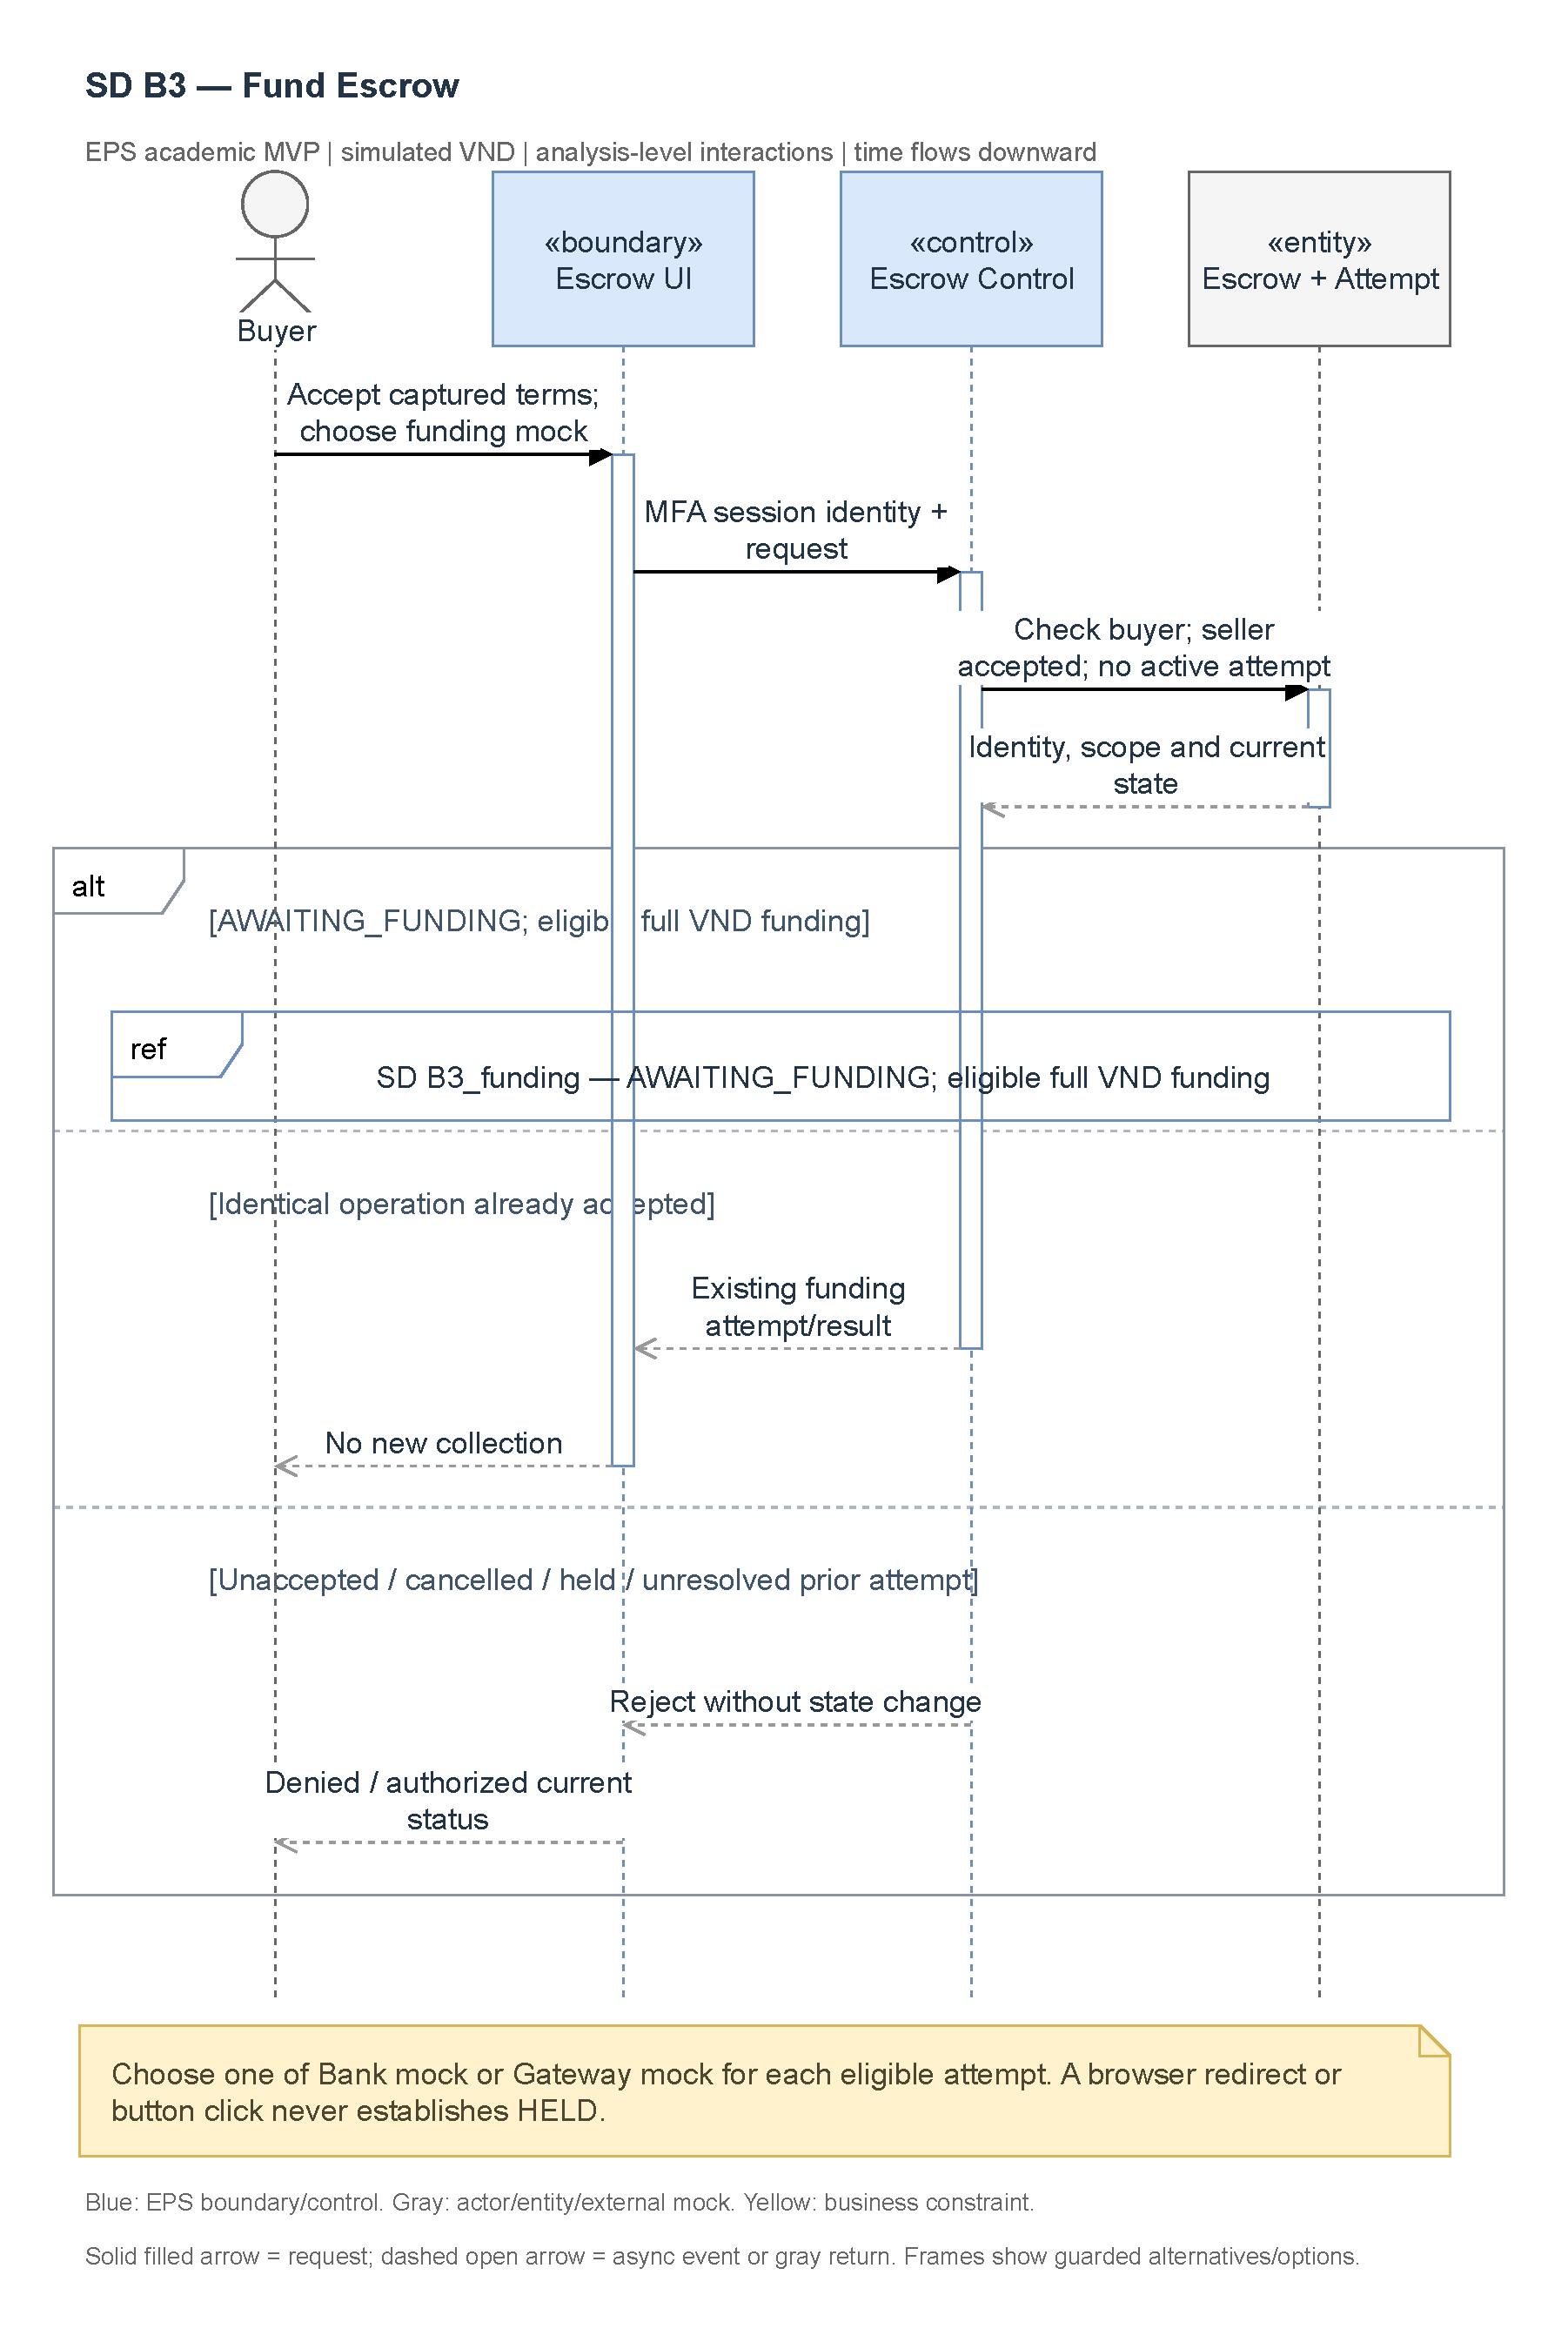
\includegraphics[width=510bp,height=700bp,keepaspectratio,clip]{diagrams/sequence/SD_B3.pdf}\caption{B3: Fund Escrow}\label{fig:sequence-b3}\end{figure}\clearpage\restoregeometry
\epsfigure{diagrams/sequence/SD_B3_funding.pdf}{B3: Fund Escrow (continued: B3\_\allowbreak{}funding)}{fig:sequence-b3-funding}
\epsfigure{diagrams/sequence/SD_B4.pdf}{B4: Confirm Acceptance and Request Release}{fig:sequence-b4}
\epsfigure{diagrams/sequence/SD_B4_outcomes.pdf}{B4: Confirm Acceptance and Request Release (continued: B4\_\allowbreak{}outcomes)}{fig:sequence-b4-outcomes}
\subsection{Seller's Use cases}
\epsfirstfigure{diagrams/sequence/SD_S1.pdf}{S1: Accept/Reject Escrow Terms}{fig:sequence-s1}
\epsfigure{diagrams/sequence/SD_S1_outcomes.pdf}{S1: Accept/Reject Escrow Terms (continued: S1\_\allowbreak{}outcomes)}{fig:sequence-s1-outcomes}
\epsfigure{diagrams/sequence/SD_S2.pdf}{S2: Record Delivery/Service Completion}{fig:sequence-s2}
\epsfigure{diagrams/sequence/SD_S2_outcomes.pdf}{S2: Record Delivery/Service Completion (continued: S2\_\allowbreak{}outcomes)}{fig:sequence-s2-outcomes}
\subsection{Admin's Use cases}
\epsfirstfigure{diagrams/sequence/SD_A1.pdf}{A1: Review and Resolve Dispute}{fig:sequence-a1}
\epsfigure{diagrams/sequence/SD_A1_decision.pdf}{A1: Review and Resolve Dispute (continued: A1\_\allowbreak{}decision)}{fig:sequence-a1-decision}
\epsfigure{diagrams/sequence/SD_A1_outcomes.pdf}{A1: Review and Resolve Dispute (continued: A1\_\allowbreak{}outcomes)}{fig:sequence-a1-outcomes}
\epsfigure{diagrams/sequence/SD_A2.pdf}{A2: Configure Escrow Policy Parameters}{fig:sequence-a2}
\epsfigure{diagrams/sequence/SD_A2_outcomes.pdf}{A2: Configure Escrow Policy Parameters (continued: A2\_\allowbreak{}outcomes)}{fig:sequence-a2-outcomes}
\epsfigure{diagrams/sequence/SD_A3.pdf}{A3: View Basic Analytics}{fig:sequence-a3}
\epsfigure{diagrams/sequence/SD_A3_outcomes.pdf}{A3: View Basic Analytics (continued: A3\_\allowbreak{}outcomes)}{fig:sequence-a3-outcomes}
\epsfigure{diagrams/sequence/SD_A4.pdf}{A4: View Audit Trail}{fig:sequence-a4}
\epsfigure{diagrams/sequence/SD_A4_outcomes.pdf}{A4: View Audit Trail (continued: A4\_\allowbreak{}outcomes)}{fig:sequence-a4-outcomes}
\epsfigure{diagrams/sequence/SD_A5.pdf}{A5: Reconcile Pending Transactions/Retry Confirmed-Failed Transfers}{fig:sequence-a5}
\epsfigure{diagrams/sequence/SD_A5_reconciliation.pdf}{A5: Reconcile Pending Transactions/Retry Confirmed-Failed Transfers (continued: A5\_\allowbreak{}reconciliation)}{fig:sequence-a5-reconciliation}
\epsfigure{diagrams/sequence/SD_A5_outcomes.pdf}{A5: Reconcile Pending Transactions/Retry Confirmed-Failed Transfers (continued: A5\_\allowbreak{}outcomes)}{fig:sequence-a5-outcomes}
\epsfigure{diagrams/sequence/SD_A5_retry.pdf}{A5: Reconcile Pending Transactions/Retry Confirmed-Failed Transfers (continued: A5\_\allowbreak{}retry)}{fig:sequence-a5-retry}
\subsection{Payment Integration's Use cases}
\epsfirstfigure{diagrams/sequence/SD_P1.pdf}{P1: Confirm Funding}{fig:sequence-p1}
\epsfigure{diagrams/sequence/SD_P1_outcomes.pdf}{P1: Confirm Funding (continued: P1\_\allowbreak{}outcomes)}{fig:sequence-p1-outcomes}
\epsfigure{diagrams/sequence/SD_P1_confirmed_receipt.pdf}{P1: Confirm Funding (continued: P1\_\allowbreak{}confirmed\_\allowbreak{}receipt)}{fig:sequence-p1-confirmed-receipt}
\epsfigure{diagrams/sequence/SD_P2.pdf}{P2: Execute and Confirm Release}{fig:sequence-p2}
\epsfigure{diagrams/sequence/SD_P2_settlement.pdf}{P2: Execute and Confirm Release (continued: P2\_\allowbreak{}settlement)}{fig:sequence-p2-settlement}
\epsfigure{diagrams/sequence/SD_P2_outcomes.pdf}{P2: Execute and Confirm Release (continued: P2\_\allowbreak{}outcomes)}{fig:sequence-p2-outcomes}
\epsfigure{diagrams/sequence/SD_P3.pdf}{P3: Execute and Confirm Refund}{fig:sequence-p3}
\epsfigure{diagrams/sequence/SD_P3_settlement.pdf}{P3: Execute and Confirm Refund (continued: P3\_\allowbreak{}settlement)}{fig:sequence-p3-settlement}
\epsfigure{diagrams/sequence/SD_P3_outcomes.pdf}{P3: Execute and Confirm Refund (continued: P3\_\allowbreak{}outcomes)}{fig:sequence-p3-outcomes}

\section{Non-functional Requirements}
The system must also meet the following non-functional requirements.

\medskip\noindent\textbf{Performance Requirements:}
\begin{itemize}
\item Target p95 response time is at most 2 seconds for internal create/query operations with 20 concurrent sessions and 1,000 simulated escrows, excluding user/provider waiting. This target has not been measured.
\item Accepted operations must return a pending status and query reference when provider settlement is unresolved.
\end{itemize}
\medskip\noindent\textbf{Operational Requirements:}
\begin{itemize}
\item Preserve pending operations, policy snapshots and provider references after interruption so reconciliation can resume without duplicate transfers.
\item Distinguish unknown outcomes from confirmed failures. Retry a payout only after confirmed failure with no money moved, preserving its direction and beneficiary.
\item Keep audit records and dashboard counts consistent with recorded escrow states.
\end{itemize}
\medskip\noindent\textbf{Security Requirements:}
\begin{itemize}
\item Require MFA for human accounts and invalidate the session on logout. Authenticate Merchant clients separately.
\item Check role, participant access and Merchant ownership on every protected operation.
\item Use TLS and authenticate provider confirmations; reject mismatched amount, currency, destination or operation references.
\item Keep the audit trail read-only and exclude passwords, MFA secrets and access tokens from logs.
\item Process repeated or concurrent money decisions once, allowing only one final release or refund.
\end{itemize}
\medskip\noindent\textbf{Cultural and Political Requirements:}
\begin{itemize}
\item Use whole VND amounts and clear delivery, acceptance and evidence terms for both goods and services.
\item Use synthetic data, label funds/providers as simulated and restrict personal and dispute evidence to authorised users.
\item Legal claims in Planning remain unverified for real deployment; the MVP makes no claim of real-money custody or regulatory approval.
\end{itemize}
